\documentclass[]{scrartcl}
\usepackage[utf8]{inputenc}
\usepackage{graphicx}
\usepackage{amsmath}

%opening
\title{Modellierung dynamischer Systeme  \\ Abgabe der Praktikumsaufgabe 1}

\author{Maria Lüdemann und Birger Kamp}

\begin{document}

\maketitle

\begin{abstract}

\end{abstract}

\section{Teilaufgabe 1}
Die zu lösende DGL ist:
$ y' = 10 - 500y + 5000x $
$ y(0) = 1 $

\subsection*{Schaltbild}
Das Simulink-Schaltbild zu dieser Gleichung ist:

\begin{figure}[htbp]
\centering
\includegraphics[width=0.7\linewidth]{a1_1_Schaltbild}
\caption{Simulink Schaltbild DGL1}
\label{fig:A1_1_Schaltbild}
\end{figure}

\subsection*{Iterationsgleichungen}
Im folgenden die Iterationsgleichungen der jeweiligen Verfahren.

\subsubsection*{Euler-Verfahren}
\begin{align}
x_{n+1} = x_{n}+h \\
y_{n+1} = y_{n}+h*f(x_{n},y_{n}) \\
y_{n+1} = y_{n}+h*(10-500y_{n}+5000x_{n})
\end{align}

\subsubsection*{Runge-Kutta-Verfahren 2.Ordnung}
\begin{align}
x_{n+1} = x_{n}+h \\
k_{1} = h*f(x_{n},y_{n}) \\
k_{1} = h*(10-500y_{n}+5000x_{n}) \\
k_{2} = h*f(x_{n} + \dfrac{h}{2},y_{n} + \dfrac{k_{1}}{2}) \\
k_{2} = h*(10-500*(y_{n} + \dfrac{k_{1}}{2})+5000*(x_{n} + \dfrac{h}{2})) \\
y_{n+1} = y_{n}+k_{2}
\end{align}

\subsection{Plot der Lösungen}
Im Folgenden sind alle Plots der Ergebnisse der Verfahren dargestellt. Es wird außerdem jeweils die Ergebnis-Differenz eines Verfahrens zur Analytischen Lösung gezeigt.
\subsubsection{h=0.001}
Das Ergebnis zeigt, dass die Verfahren bis x=0.01 sehr ähnliche Ergebnisse liefern, und haben eine max. Differenz von ca. 0.12. Danach laufen alle Kurven kongruent.
\begin{figure}[htbp]
\centering
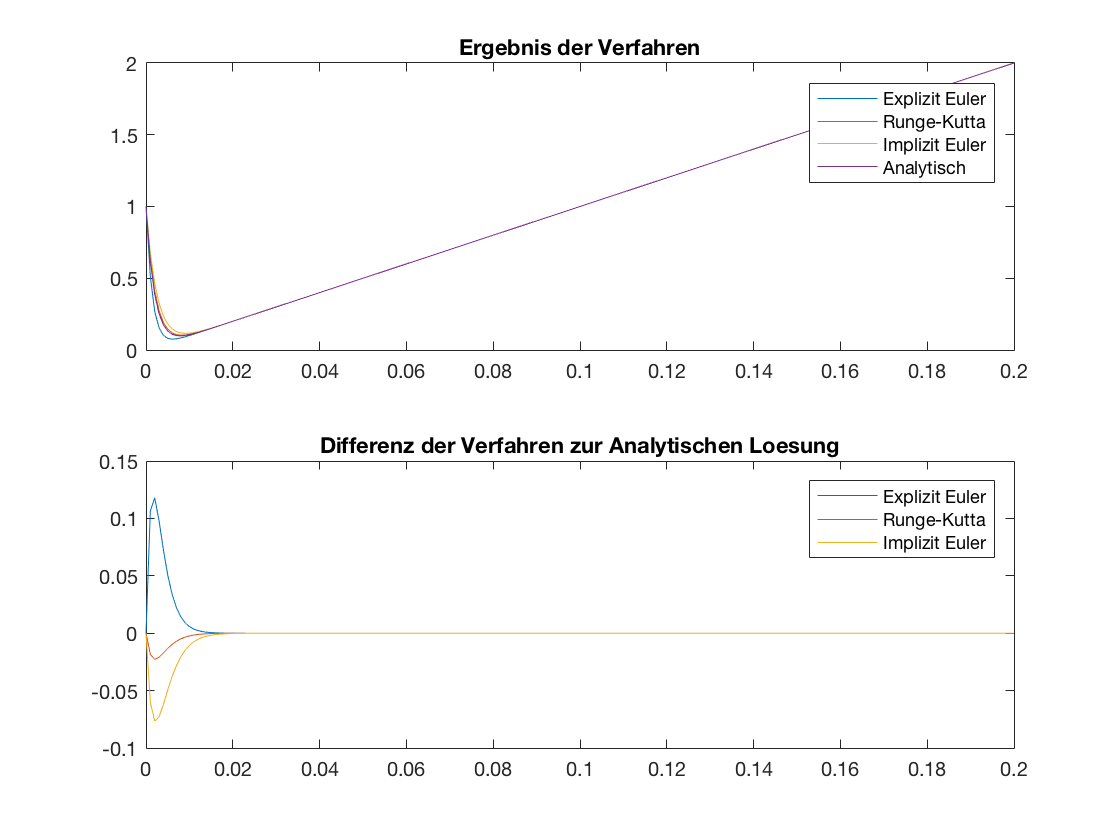
\includegraphics[width=1\linewidth]{a1_1_1}
\caption{h=0.001}
\label{fig:a1_1_1}
\end{figure}

\subsubsection{h=0.003}
Das Ergebnis zeigt, dass die Verfahren bis ca. x=0.03 unterschiedliche Ergebnisse liefern. Die Ergebnisse des Runge-Kutta-Verfahrens verlaufen bis ca. x=0.03 nahezu parallel zur analytischen Lösung. In diesem Wertebereich liefert das explizite Euler-Verfahren sehr schwankende Werte. Ab ca. x=0.03 laufen alle Kurven kongruent.
\begin{figure}[htbp]
	\centering
	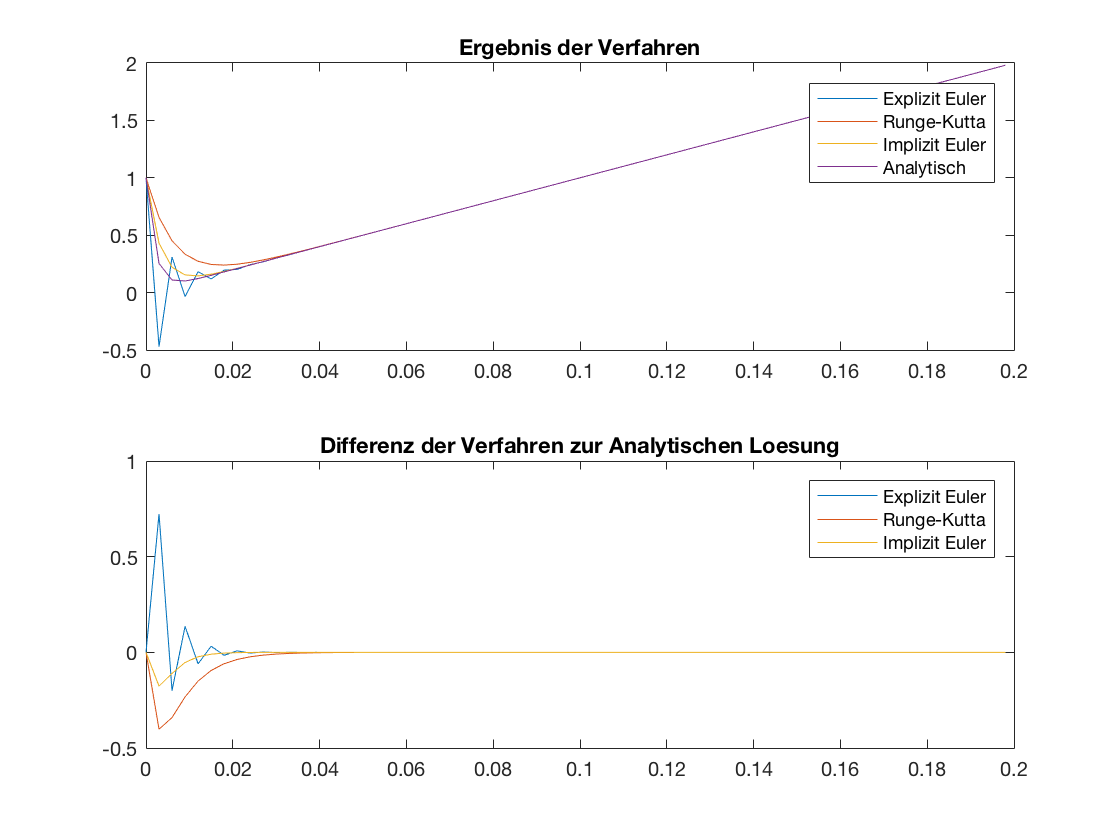
\includegraphics[width=1\linewidth]{a1_1_2}
	\caption{h=0.003}
	\label{fig:a1_1_2}
\end{figure}

\subsubsection{h=0.004}
Bis ca. x=0.01 laufen alle Kurven unterschiedlich. Ab dort laufen die Kurven des Runge-Kutta-Verfahrens und der analytischen Lösung kongruent. Während der ganzen Laufzeit liefert das explizite Euler-Verfahren sehr schwankende Werte, die sich mit einer Differenz von +/- 1 in der Nähe der analytischen Lösung befinden.
\begin{figure}[htbp]
	\centering
	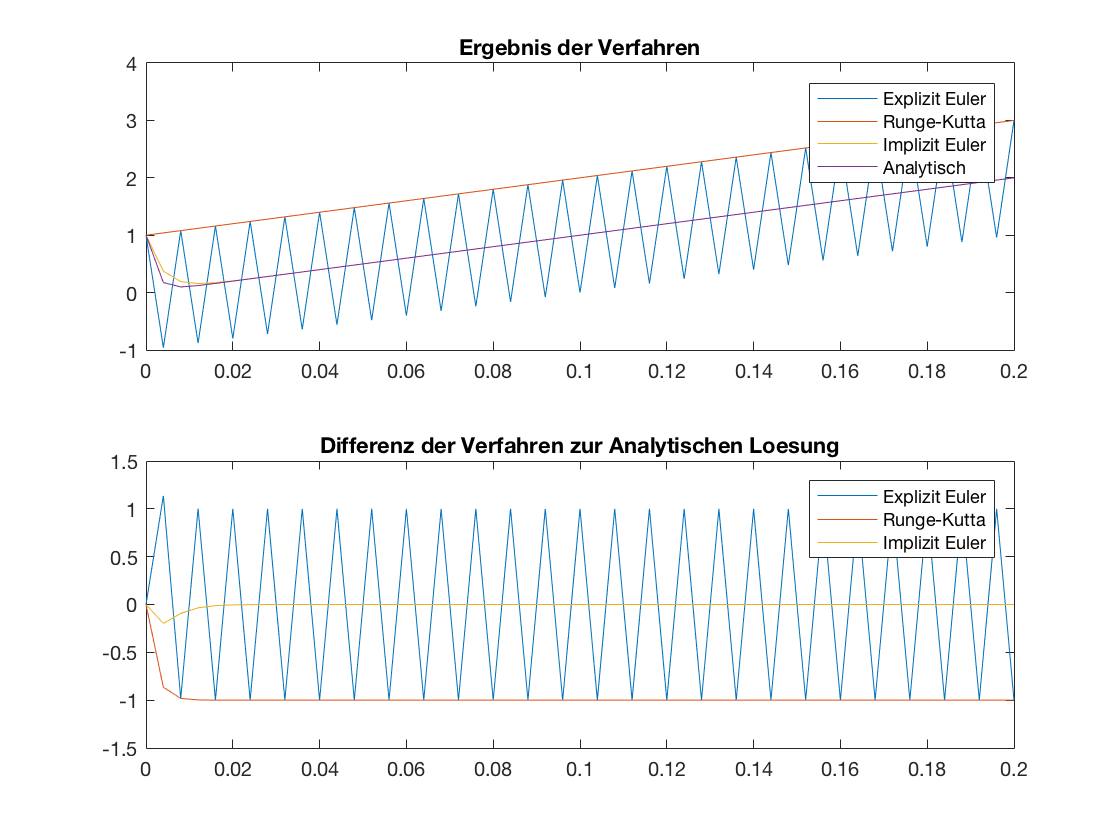
\includegraphics[width=1\linewidth]{a1_1_3}
	\caption{h=0.004}
	\label{fig:a1_1_3}
\end{figure}

\subsubsection{h=0.005}
Bis ca. x=0.15 laufen alle Kurven kongruent. Ab dort schwanken die Werte des expliziten Euler-Verfahrens mit einer Differenz von ca. +/- 0.1 um die Werte der analytischen Lösung. Die Werte des Runge-Kutta-Verfahrens hingegen werden ab ca. x=0.15 exponentiell größer.
\begin{figure}[htbp]
	\centering
	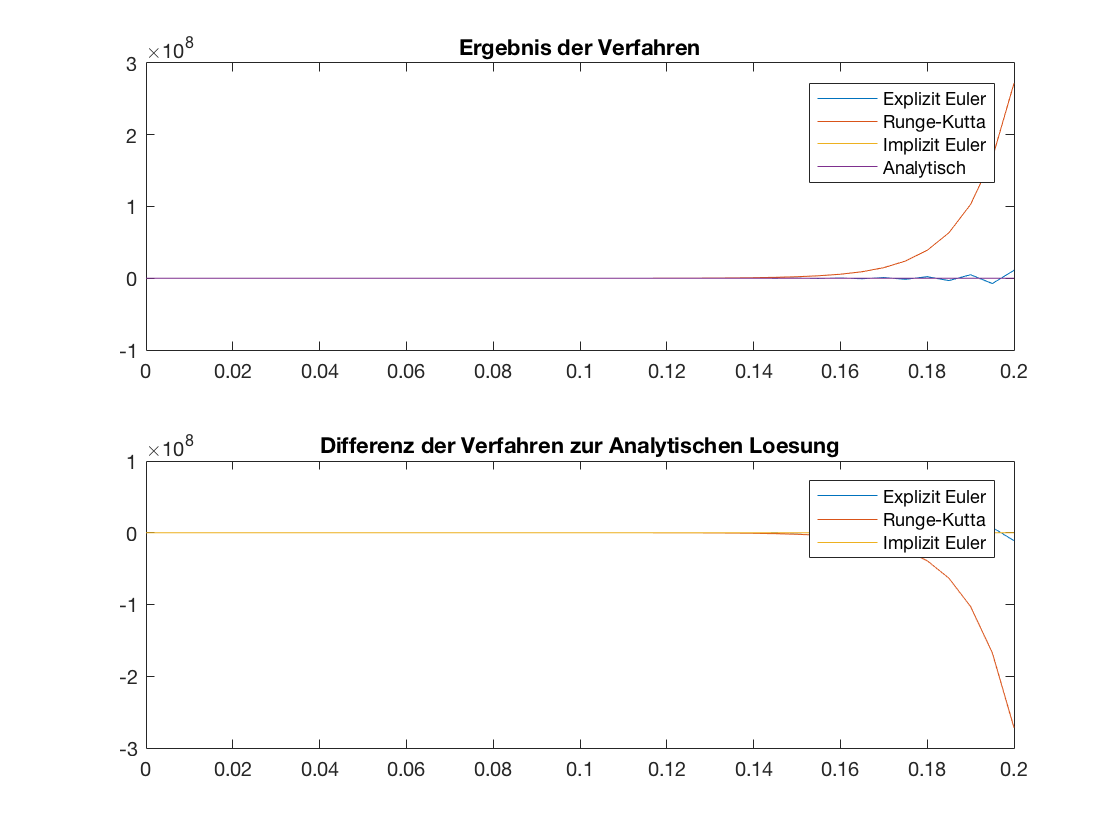
\includegraphics[width=1\linewidth]{a1_1_4}
	\caption{h=0.005}
	\label{fig:a1_1_4}
\end{figure}

\subsection{Interpretation der Ergebnisse}
\subsubsection{Explizites Euler-Verfahren}
Die Ergebnisse zeigen, dass dieses Verfahren bei einer geringen Schrittweite genauere Ergebnisse liefert. Allerdings wird dadurch die benötigte Rechenzeit erhöht.

\subsubsection{Runge-Kutta-Verfahren 2ter Ordnung}
Die Ergebnisse zeigen, dass dieses Verfahren bei einer geringen Schrittweite genauere Ergebnisse liefert. Allerdings wird dadurch die benötigte Rechenzeit erhöht.


\end{document}
